\documentclass[10pt, a4paper]{article}
\usepackage[finnish]{babel}
%\usepackage[landscape, margin=0.7in]{geometry}
\usepackage[print]{booklet}

\usepackage{titlesec}
\usepackage{graphicx}
\usepackage[utf8]{inputenc}
\usepackage{multicol}
\usepackage[osf]{mathpazo} % URW Palladio + Old-style numerointi
\usepackage{pgfornament}
\usepackage{float}
\usepackage[11pt]{moresize}
\usepackage[export]{adjustbox}
\raggedcolumns

\titleformat*{\section}{\normalsize\bfseries}

\setlength{\parindent}{0pt}
\setlength{\parskip}{0.25cm}
\setlength{\columnsep}{.5cm}
\setpdftargetpages
\addtolength{\oddsidemargin}{.4in}
\addtolength{\evensidemargin}{-0.5in}

\begin{document}
\pagenumbering{gobble}
\begin{center}


\vspace*{1.5cm}
\textbf{\sc\Huge Yöjäynä-sitsit 2022}


\vspace{0.2cm}
%\rule{2cm}{1pt}

\pgfornament[scale=0.15]{80}
%viiva
\pgfornament[scale=0.25]{58}
%viiva
\pgfornament[scale=0.15]{80}

\vspace{0.2cm}

\sc\Large Lorem ipsum

\sc\Large Smökki 18.12.2022

\vspace{1cm}


\includegraphics[scale=1.0]{kuvat/YJ22logo.png}

\end{center}

\pagebreak
\pagenumbering{arabic}
\begin{multicols}{2}

%%% v Lauluja v Lauluja v Lauluja v Lauluja v Lauluja v Lauluja v %%%

\begin{flushleft}

\section{Hyvät ystävät}
Hyvät ystävät juhla voi alkaa\\
Sankarille me nostamme maljaa\\
:,: Tääll’ ei juodakaan kolmosen \\
kaljaa.\\
Meille viihdyn suo samppanja vaan~:,: 

Hauska juomia kurkkuun on suistaa\\
Siten teekkariaikoja muistaa\\
:,: Yhteinen juomalaulumme luistaa \\
Juhlamieli on parhaimmillaan :,:

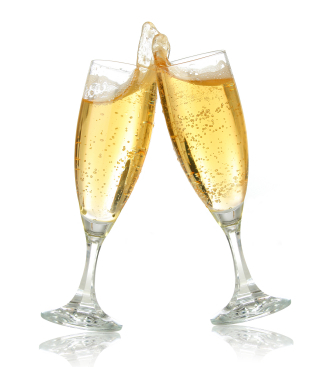
\includegraphics[scale=.40]{kuvat/skal.jpg}

\section{Etanoli-Tetris}

Pohjalle pistelen pullosta koskista\\
Paan sen seuraan shampanjaa\\
Poistan tyhjiä kelpo kaljalla\\
Viski jo kuplat vaimentaa

Pakkailen boolia, alkomahoolia\\
päin mun suolen seinustaa\\
Pintaan täyttäen, tietä näyttäen\\
Kurkusta kaatuu gambinaa

Siideri, lonkero, jägeri, katkero\\
Saan jo jallun paaluttaa\\
Ahtaan tunnelman rommiryypyllä\\
Gin-zipin tiiviin kippaan taa

Kompressoin konjakit, punkut ja valkkarit\\
Suu jos kuivaa, ferraa paan\\
Hehkuviini tai portti fiini ja \\
konjakki vodkaa kerrostaa

Absinttihaaveissa, pontikkasaaveissa\\
uin, ja lastaan maltaista\\
Tuuba mielessä, punssi kielessä\\
Kittailen grappaa tuopista\\

Tiiviiksi taistellen, tiuhasti maistellen\\
voin tän kaiken mahduttaa\\
Tukkoon laittaen, kaksin taittaen\\
Viel parit pystyy kellottaa

\section{Se kolmas vesilaulu}

Vettä kun juoda saa\\
Se voipi pelastaa,\\
ei iske känni,\\
ei ala ränni.\\
Vesi on herkkua,\\
kostuttaa kurkkua.\\
Ei tarvii dokata,\\
eikä voi mokata.\\
Raitis on olo,\\
ei keuli mopo.\\
Aamulla ei\\
ole krapulaa.

\section{Elomme päivät}

Elomme päivät epäselvät\\
kohtalo kova suonut on.\\
:,: Kun eilen tulin tänään kotia\\
ja tänään tulen huomenna. \\
Huomenta! :,:

Jumalauta täällä sammutaan!\\
Siskot, veljet, tulkaa auttamaan!\\
:,: Me baarikaapin näämme ja sen valtaamme  \\
ja kossupullon huiviin heitämme. Perkele! :,:

%\section{Tunnetko jo Lapparin}

Oot vielä ilman juomaa\\
Tää ilta selvä on \\
Mut kun mä saavun kautta Alepan, niin lavan meille tuon \\
Kun tölkit ensimmäiset \\
Nostetaan boksista \\
Niin yötä myöten yksi kerrallaan \\
Se boksi tuhotaan 

:,: Tunnetko jo Lapparin? \\
Sen tunnen viljaisen \\
Juo pohjaan vaan \\
Me Kultaa huuhdotaan  \\
Viel yhdet korkataan :,:

\pagebreak

\section{Eurovision}

Ranskassa juodaan viiniä\\
Saksassa olutta, Venäjällä vodkaa.\\
Suomessa juodaan kaikkea,\\
Siis malja sille nostakaa!

Norjassa poltetaan kirkkoja\\
Saksassa kirjoja, Venäjällä vodkaa.\\
Hollannissa poltetaan kaikkea,\\
Siis sätkä sille käärikää!

Norjassa syödään lunta\\
Ruotsissa loskaa, Venäjällä paskaa.\\
Tampereella syödään kaikkea,\\
Siis perseet sinne kääntäkää!

Ennen oli miehet rautaa\\
ja laivat oli laivantekoaineesta tehty.\\
Nykyään on miehet puuta,\\
ja laivat ovat merenpohjassa. POHJASSA!

\section{Helan går}

\textit{Soolo:}\\
En liten fågel satt en gång\\
Och sjöng I furuskog.\\
Han hade sjungit dagen lång\\
Men dock ej sjungit nog.

Och strupen torkat vid hans gom\\
förtröstan stämman bar.\\
Vad sjöng den lilla fågeln då?

\textit{Kaikki:}

JO!

:,: Helan går,\\
sjung hopp-falderallan-lallan-lei! :,:\\
Och den som inte helan tar,\\
Han ej heller halvan får.\\
Helan går!\\
sjung hopp-falderallan-lei!

\vspace{0.3cm}

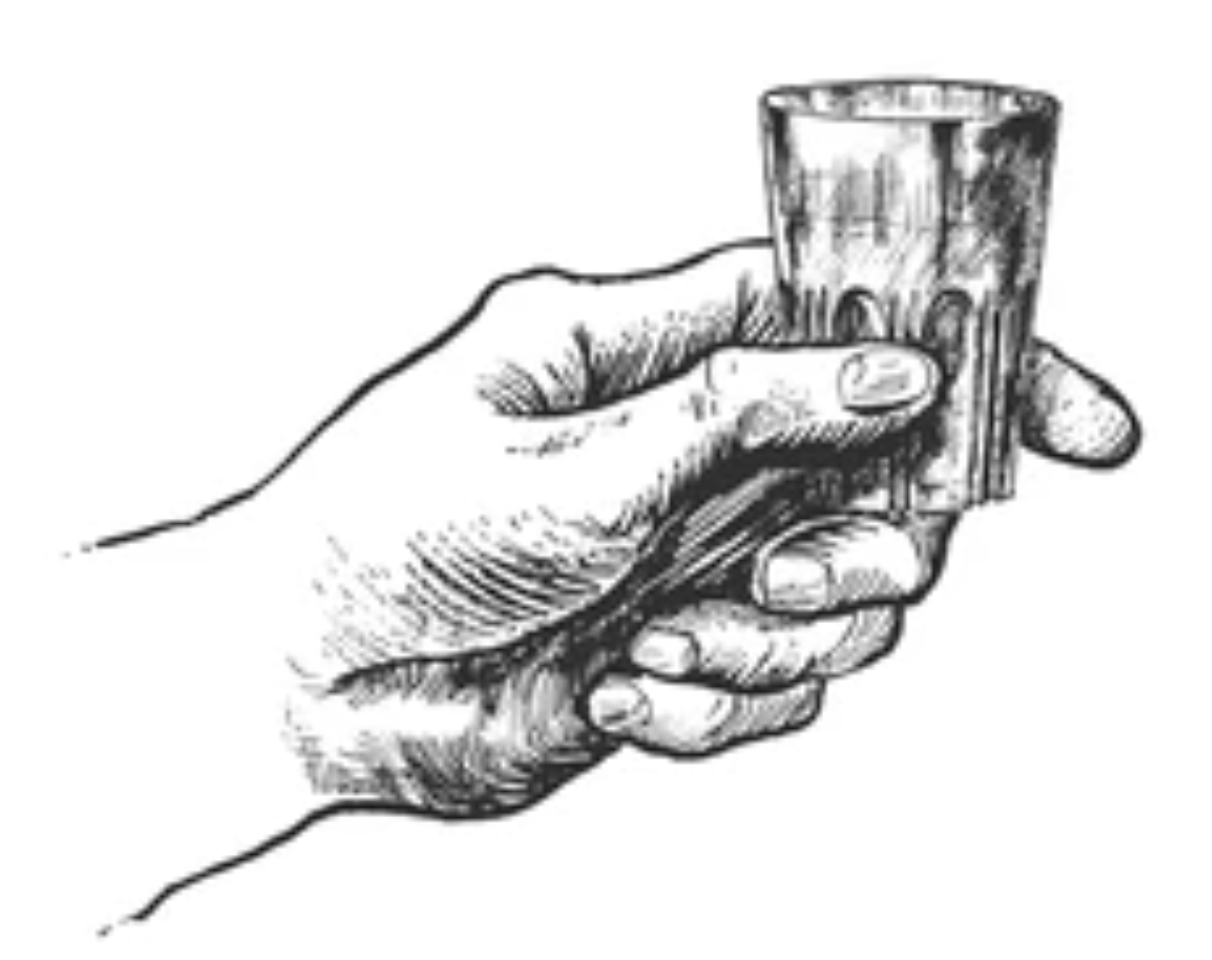
\includegraphics[scale=.1, center]{kuvat/shot.png}

\columnbreak

\section{Ko-Ko-Koskenkorvaa}
%\textit{Melodia: Volga}

Ko-ko-ko-kosken-ko-ko-ko-korvaa,\\
siitä aina kunnon rä-kä-kä-kännit saa.\\
Ko-ko-ko-kosken-ko-ko-ko-korvaa,\\
siitä aina kunnon rä-kä-kä-kännit.\\
aina kunnon rä-kä-kä-kännit,\\
aina kunnon rä-kä-kä-kännit saa!

La-la-la-lappeen Ra-ra-ra-rantaan,\\
siellä aina kunnon rä-kä-kä-kännit saa.\\
La-la-la-lappeen Ra-ra-ra-rantaan,\\
siellä aina kunnon rä-kä-kä-kännit,\\
aina kunnon rä-kä-kä-kännit,\\
aina kunnon rä-kä-kä-kännit saa!\\

We-we-we-Westendinrantaan,\\
siellä aina isin bemarissa saa.\\
We-we-we-Westendinrantaa,\\
siellä aina isin bemarissa,\\
aina isin bemarissa,\\
aina isin bemarissa saa!

O-O-O-Otaniemenrantaan,\\
siellä teekkari ei solussansa saa.\\
O-O-O-Otaniemenrantaan,\\
siellä teekkari ei solussansa,\\
teekkari ei solussansa,\\
teekkari ei solussansa saa!

Bo-bo-bo-Bodom järven rantaan\\
Siellä aina kunnon telttahoidon saa\\
Bo-bo-bo-Bodom järven rantaan\\
Siellä aina kunnon telttahoidon\\
Aina kunnon telttahoidon\\
Aina kunnon telttahoidon saa!

Sa-sa-sa-saunaa Ga-Ga-Ga-Gambinaa,\\
Sillä aina kunnon saunalöylyt saa!\\
Sa-sa-sa-saunaa Ga-Ga-Ga-Gambinaa,\\
Sillä aina kunnon saunalöylyt\\
aina kunnon saunalöylyt\\
aina kunnon saunalöylyt saa!
\vspace{0.2cm}

\pagebreak

\section{Tänään otetaan}
:,: Tänään otetaan, tänään otetaan\\
helevetin paljon viinaa! :,:\\
:,: Huomenna on, huomenna on\\
helevetin kova krapula. :,:

:,: I dag ska vi ta, i dag ska vi ta\\
helvetes mycket brännvin! :,:\\
:,: I morgon ska vi ha, i morgon ska vi ha\\
helvetin kova krapula! :,:

:,: Tänä võtame, tänä võtame\\
kuradima palju viina. :,:\\
:,: Homme meil on, homme meil on\\
kuradima kova pohmakas. :,:

:,: Tonight we shall get, tonight we shall get\\
Absolutely fucking hammered :,:\\
:,: Tomorrow we shall have, tomorrow we shall have\\
Hangover beyond reason :,:

\vspace{-0.4cm}

\section{Viljaviinaa}
Viljaviinaa, maistetaan,\\
Viljaviinaa, siitä ryypyn saa!\\
Viljaviinaa, lauletaan,\\
sillä kaukaiset aarteet me aukaistaan.

Viljaviinaa, maistetaan,\\
Viljaviinaa, siitä ryypyn saa!\\
Viljaviinaa, trallalaa,\\
sillä kaukaiset aarteet me aukaistaan.

Leijonaa, toiset meille haluaa suosittaa,\\
Koskenkorvaa, Vaakuna-viinaa.\\
Kuinka on, jos Wyborowa sitsimme juhlistaa?\\
Onko Tasavalta, Alku-viina,\\
Metsästäjän, Kalastajan\\
Perinne, Tyrnävän, Smirnoff parempaa?

(Skål!)

Viljaviinaa,\\
Viljaviinaa, maistetaan\\
Viljaviinaa, siitä ryypyn saa,\\
Viljaviinaa, trallalaa\\
Sillä äänemme myös me aukaistaan.\\
Absolut!

\section{Sörkan sällit}

Sörnai gusha nietu molotova,\\
Sörnai gusha herba moskova,\\
:,: Njet, njet bonimai votvot risubuska,\\
Dara zeva votvot harashoo :,:

Isä Stalin, äiti Hrushtsheva\\
Isgi silmää ginihibragas,\\
:,: Oi, oi oisiba vodkaa ollut heillä\\
Oisi isgu gäynyd alemmas :,:

Tuoksuu tuomet, syreenit ja ruusut,\\
Tuoksuu tuolla Volgan randamill,\\
:,: Ai, ai, kaunis kulta Kaditzusha\\
Tuoksuu tunteet rindas rindamil :,:

Siellä missä versoaapi vilja,\\
Siellä kasvoi kaunis Katjuska.\\
:,: Katjuskalla komiat on keuhkot,\\
Basga haisee Nevan rannalla :,:

Oon vain köyhä kolhoosinainen,\\
Ei oo mulla yhtään ystävää.\\
:,: Ei ole lehmää eikä ole lammasta\\
Eikä suussa yhtään hammasta :,:

Siperian lakeus on suuri,\\
Sonja siellä lunta lapioi.\\
:,: Sonjalla kävi hiton huono tuuri kun\\
Länsituuli uutta lunta toi :,:

Olen köyhä poika Petroskoista,\\
Ei oo mulla yhtään ystävää.\\
:,: Sirppi ja vasara ne taivahalla loistaa,\\
Basga haisee, balalaikka soi :,:

%\section{Pienet aaltolaiset}

:,: Pienet teekkarit, pienet teekkarit niin lystikkäitä on :,:\\
Ei naisia, ei naisia, ei naisia milloinkaan.\\
Ei naisia, ei naisia, ei saa ne milloinkaan.

:,: Pienet kylterit, pienet kylterit niin lystikkäitä on :,:\\
:,: Ei sielua, ei sielua, ei sielua ollenkaan :,:

:,: Pienet artistit, pienet artistit ne sekaisin vaan on :,:\\
:,: Ei fyffeä, ei fyffeä, ei fyffeä laisinkaan :,:

\pagebreak

\section{Internationalen}

Mera brännvin i glasen,\\
mera glas på vårt bord,\\
mera bord på kalasen,\\
mera kalas på vår jord.\\
Mera jordar kring månen,\\
mera månar kring Mars\\
mera marscher till Skåne,\\
mera Skåne, bevars!

Lisää viinaa mun lasiin,\\
lisää laseja pöydälle,\\
lisää pöytiä näihin juhliin,\\
lisää juhlia kansalle.\\
Lisää kansaa Suomeen,\\
lisää Suomea päälle maan,\\
lisää maata Suomelle,\\
marssitaan Karjalaan, Karjalaan!

\section{Lärvit}

:,: Lärvit, lä-lä-lä-lärvit, 
lä-lä-lä-lärvit, nyt otetaan! :,: 
 
Kun tänään otan monta tuoppia kuohuvaa, 
niin hyvän olon siitä saan. 
Ja siihen päälle vedän putelin koskista, 
niin siitä vasta kone käynnistyy! 
 
:,: Lärvit, lä-lä-lä-lärvit, 
lä-lä-lä-lärvit, nyt otetaan! :,: 
 
Imperiumin vastaisku! 
Kraa-kraa-kraa-kraa-pula-kraa-pula, 
kraa-kraa-kraa-kraa-pula-kraa-pula. 
Kraa-kraa-kraa-kraa-kra-kra-pula, 
kra-kraa-kraa-kra-kra-pula, 
kra-kraa-kraa-pula-kraa-pula. 
 
Jedin paluu! 
:,: Lärvit, lä-lä-lä-lärvit, 
lä-lä-lä-lärvit, nyt otetaan! :,: 
 
Duel of the Fates! 
// Kaikki 
Koskenkorvaa, koskenkorvaa, koskenkorvaa... 
// Soolo 
Jallu, Kossu, Kalja, Ferra...

\columnbreak
\section{Drunken Sailor}
What shall we do with a drunken sailor (x3)\\
early in the morning

Hooray and up she rises (x3)\\
early in the morning

Shave his belly with a rusty razor (x3)\\
early in the morning

Hooray...

Put him in a long boat till he's sober (x3)\\
early in the morning

Hooray...

Put him in the bed with a captain's daughter (x3)\\
early in the morning

Hooray... %eng

\section{Hei vahtimestari}

:,: Hei vahtimestari,\\
tule, täytä lasini,\\
vie tyhjät pullot pois :,:\\
:,: Kyllä enemmänkin juodaan,\\
jos vain lisää tuodaan,\\
ja laskut maksetaan, jos jaksetaan. :,:


:,: Hei, vahtimestari,\\
tule täytä lasini,\\
vie kuolleet phuksit pois! :,:\\
:,: Ja jos mä kerran kuolen,\\
niin kilta pitää huolen,\\
ett’ Pokkamonttuun minut haudataan. :,:


:,: Hei, vahtimestari,\\
tule täytä suoleni,\\
se onkin minun paras puoleni. :,:\\
:,: Ja kun mä kerran kuolen,\\
niin kilta pitää suolen,\\
se vuosijuhlalahjaks’ annetaan. :,:

\pagebreak

\section{Silja Line Special}
Tahtoisin ginitonicin, ginitonicin\\
Tai sitten minttufernetin, minttufernetin\\
Kyll’ kelpais kossuvissykin, kossuvissykin\\
Nyt ryypätään, nyt ryypätään

Jos saisin, mitä tekisin, mitä tekisin?\\
Kyll’ varmaan jotain keksisin, jotain keksisin,\\
tai sitten kotiin juoksisin, kotiin juoksisin.\\
Nyt jänistää, nyt jänistää.

Kyll’ pojat eilen häpesin, eilen häpesin,\\
kun yhden tytön tapasin, tytön tapasin,\\
ja sitten homman mokasin, homman mokasin.\\
Nyt hävettää, nyt hävettää.

On mulla naama valkoinen, naama valkoinen\\
ja maistuis olut huurteinen, olut huurteinen\\
Juon sitä kolpakollisen, kolpakollisen\\
ja oksennan, yli laidan.

\section{Otaniemi Shangri-La 2020}
Pilalla on vanha kunnon Otaniemen henki.\\
Entisaikaan riitti Gambina ja puistonpenkki.\\
Hurrahuhhahhei! Krääsäpuodit, kuntosalit.\\
Kaikenlaista turhaa paskaa tänne työnnetään.

Otaniemen kaduilla ei kävelemään päästä,\\
kun viittä vitun metriä ei voi katutöiltä säästää.\\
Hurahuhhahhei! Kuka tämän suunnitteli?\\
Paras jalankulkuväylä on nyt pyörätie.

On metro valmis, mutta hemmo meni silti pieleen.\\
Asemien ruuhkat lienee päättäjille mieleen.\\
Hurahuhhahhei! Muka automaatti korvaa.\\
Nauraa varikstetkin Espoon metrimetrolle.

Taiteilijat simputusta lehtorilta sietää:\\
jos ruman paidan neuloo,\\
niin se uran loppuu tietää.\\
Hallelujahei! Toista se on teekkareilla.\\
Oppii prujaamaan, niin töitä saa ja valmistuu.

St1 porallaan maan järisemaan laittaa.\\
Kovasti se Kulosaaren rahakkaita haittaa.\\
Hurahuhhahhei! Kyllä tietää insinööri:\\
"Tämä toinen reikä meneekin jo helpommin"

Korona kun iskee, niin ei Aalto-sali täyty.\\
Eipä siellä aiemminkaan istumassa käyty!\\
Hallelujahei! pandemian digiloikka.\\
Täällä proffat käyttää vielä piirtoheitintä.

Kun huippuyliopistoa Otaniemen luodaan,\\
teekkarine yksiöissä Jallua vaan juodaan.\\
Hurahuhhahhei! Melkein Alko saatin tyhjäks.\\
Kiitos siitä! Nyt on Aalto vihdoin Shangri-La.

\columnbreak

\section{Jos eukkosi kieltää}

Jos eukkosi kieltää sua juomasta,\\
niin juo, niin juo.\\
Jos kieltää sua viinoja tuomasta,\\
niin tuo, niin tuo.\\
Mutt' juomasta älä sinä milloinkaan lakkaa,\\
vaan hanki sinä itselles' parempi akka,\\
Ja juo ja laula, ja juo ja laula,\\
ja juo ja laula, ja juo ja laula ja…

Trink, trink, Brüderlein trink\\
lass doch die Sorgen zu Haus!\\
Trink, trink, Brüderlein trink,\\
leere dein Glas mit mir aus!

Meide den Kummer und meide den Schmerz,\\
dann ist das Leben ein Schertz,\\
Zu lieber Augustin!\\
Kauf dir ein Auto und fahr gegen Baum,\\
dann ist das Leben ein Traum!

Upseerit sotia taistelee,\\
ja juo, ja juo,\\
Ja teltassa viinoja maistelee,\\
ja juo, ja juo.\\
Kun taistelun melskeissä pyssyt ne paukkaa,\\
niin upseerit välillä pullosta naukkaa,\\
Ja juo ja laulaa ...

Maisterit koulussa opettaa,\\
ja juo, ja juo,\\
ja illalla tuntinsa lopettaa,\\
ja juo, ja juo.\\
Kun päivällä saksaa ja matikkaa jauhaa,\\
niin illalla raitilla räyhää ja pauhaa!\\
Ja juo ja laulaa ...
\vspace*{1.2cm}

\section{My Favourite Drinks}

Negroni, Manhattan, Tequila sunrise;\\
Gin Tonic, Blue Angel, a vodka on ice;\\
Campari orange, Ferrari, Tom Collins;\\
these are a few of my favourite drinks!

Screwdriver, Grasshopper, Apple Martini;\\
Black russian, White russian! Long island ice tea;\\
Little green fairies absinthe on their wings;\\
These are a few of my favourite drinks;

When the glass breaks;\\
or my hand shakes;\\
when I'm feeling sad;\\
I mix up a few of my favourite drinks,\\
and then I don't feel so bad! %eng
%change this to fast food

\section{Bittilaulu}
0000 0001\\
0010 0011\\
0100 0101\\
0110 0111

1000 1001\\
1010 1011\\
1100 1101\\
1110 1111

\columnbreak
\section{No onkos tullut joulu}
No onkos tullut kesä nyt talven keskelle?\\
:,: Ja laitetaankos pesä nyt pikkulinnuille? :,:

Jo kuusi kynttilöitä on käynyt kukkimaan.\\
:,: Pimeitä talven öitä nyt ehkä valaistaan. :,:

Ja vanhakin nyt nuortuu kuin lapsi leikkimään.\\
:,: Ja koukkuselkä suortuu, nyt kaikk' on mielissään. :,:

Lumi on jo peittänyt kukat laaksosessa,\\
järven Aalto jäätynyt talvipakkasessa.\\
Varpunen pienoinen, syönyt kesäeinehen,\\
järven Aalto jäätynyt talvipakkasessa.

:,: Joulu on nyt, joulu on nyt,\\
kattilat täynnä puuroo. :,:\\
:,: Nyt sitä saa, nyt sitä saa,\\
vatsansa täyteen puuroo. :,: 

\section{Vinetto}
\textit{Melodia: Petteri Punakuono}

Muistat Chardonnayn,\\
Beaujolais'n, Tokajin varmaan\\
ja Tempranillot ja Martinin karvaan.\\
Mutta viini tää\\
sulta usein unhoon jää:

Vinetto-mausteviini\\
ruskea on väriltään.\\
Liene ei liian fiini\\
Vinettomme kellekään.\\
Haukkuivat toiset illoin\\
tärpätiksi pilkaten\\
Tuosta vain saikin\\
silloin teekkarimme aattehen:

"Vuosijuhla pitkä on,\\
puhemaraton.\\
Vinetto vois mukanaan\\
viedä sieltä humalaan!"

Vinetto siitä asti,\\
povarissa matkaten\\
nousuun saa joutuisasti\\
:,: juhlamielen iloisen! :,:\\
Juhlamielen iloisen!

\section{Syphilis}
Syphilis,\\
it just started with a simple kiss\\
Now it even hurts to take a piss\\
Oh how did I get syphilis?

Yesterday\\
My cock was always coming out to play\\
Now it needs two weeks to hide away\\
Oh I believe in yesterday

Why her box was sick\\
I don't know, she wouldn't say\\
Now my dripping dick\\
won't get hard like yesterday-ay-ay-ay

Leprosy,\\
I'm not half the man I used to be\\
Now my fingertips are leaving me\\
Oh I believe I've leprosy.

Amputees.\\
You don't even have to spread their knees,\\
You can slide it in and out with ease,\\
Oh I believe in amputees.

Why, I had to come,\\
I don't know she wouldn't blow.\\
I stayed in too long.\\
Now I long for birth control.

\pagebreak

\input{laulut/alla-borde-känna-till.tex}

\section{Santa Lucia}
Jag i silentio\\
gör promenado,\\
nocturno solo\\
in Esplanado.\\
Jag där med gran favor\\
väntar min pia.\\
Santa Lucia, Santa Lucia.

Con vehementio\\
slår jag rivalen\\
och etablerar\\
grande scandale.\\
Polisconstabelo\\
skurken befria,\\
Santa lucia, Santa lucia

Jag skrek fortissimo\\
"Släpp mig för Phano!"\\
Han skrek crescendo:\\
"Parlo non guano!"\\
Jag in arresto förs,\\
å infamia.\\
Santa lucia, Santa lucia

Å hårde destiné,\\
här in obscuro\\
gråter jag lacrymæ,\\
ödet är duro.\\
Önskar al diavolo,\\
amore mia,\\
Satans Lucia, Satans Lucia!


\input{laulut/valomerkin-jälkeen}

\pagebreak


\section{Muinaisten valssi}


Saimaan saaressa pikkuinen torppa,\\
uhraa portailla kultisti Miikkulainen,\\
mutta pintaan ei nouse kuin norppa,\\
on pettymys melkoinen.\\
Aallon alla se suunnisti kutsujan luo,\\
sille tuttua tutumpi on messu tuo.\\
Laulu kertoo näin mitä on yksin kun jää,\\
hyvin hylje sen ymmärtää.

Uhrata enää ei Cthulhulle päitä,\\
maailma modernisoitunut on.\\
Muinaisjäänteitä viiksekkäitä,\\
mies sekä hylje kumpikin on.

Saimaan saaressa pikkuinen torppa,\\
sinne muinaisten kulttinsa tahtonut ei.\\
Yksin kultisti jäi kuten norppa,\\
myös sen mestarin kohtalo vei.\\
Suuri Saimaa mut sata on hylkeitä vaan,\\
kohta jäljellä ei ehkä ainuttakaan.\\
Uhriveistänsä teroittaa Miikkulainen,\\
aatos mieleessään hirmuinen.

Uhrata enää ei Cthulhulle päitä,\\
maailma modernisoitunut on.\\
Muinaisjäänteitä viiksekkäitä,\\
mies sekä hylje kumpikin on.

Saimaan saaressa pikkuinen torppa,\\
karjuu loitsuja kultisti Miikkulainen.\\
Uhrikivellä hengetön norppa,\\
makaa hiljalleen kylmentyen.\\
Suuri Saimaa ja alta sen lainehien,\\
nousee kauhu niin vanha ja lonkeroinen.\\
Niin on kohtalo norpan kuin Miikkulaisen,\\
olla sukunsa viimeinen.

Viimeinkin uhrataan Cthulhulle päitä,\\
maailmaan palannut muinainen on.\\
Lounaaksi syötyjä pölkkypäitä\\
mies sekä hylje kumpikin on.
\section{Minnet}
Minne! Jag har tappat mitt minne!\\ 
Är jag svensk eller finne?\\
Kommer inte ihåg ...

Inne! Är jag ut eller inne? \\
Jag har luckor i minne, \\
sån’där små alkohol.

Men besinn’er, man tätar med det brännvin man får, \\
fasän minnet och helan går. \\

Minne? Muisti hävis’, mutt’ minne? \\
Juhlista selvisimme \\
- muistikatkoja on.

Minne? Lähtisin vaikka minne, \\
kunhan selvittäisimme \\
mitä tapahtunut on

Mutta tiedän mä keinon \\
mikä auttaapi tuo: \\
ota ryyppy, ja muistis’ juo!

\section{Hullu kirvesmies}

Illalla, kun mielipuoli kirveen saa,\\
hän johdattaa mut aitan taa,\\
siellä missä aivokoppa aukeaa\\
ja verikin on punaisin.

:,:Nauraen lyö hullu niskan taa,\\
tunnen sen jo veri tirskahtaa.\\
Vaikk’ on taju himmennytkin,\\
hullu hakkaa vielä nytkin\\
niskantynkää verta pursuvaa.:,:


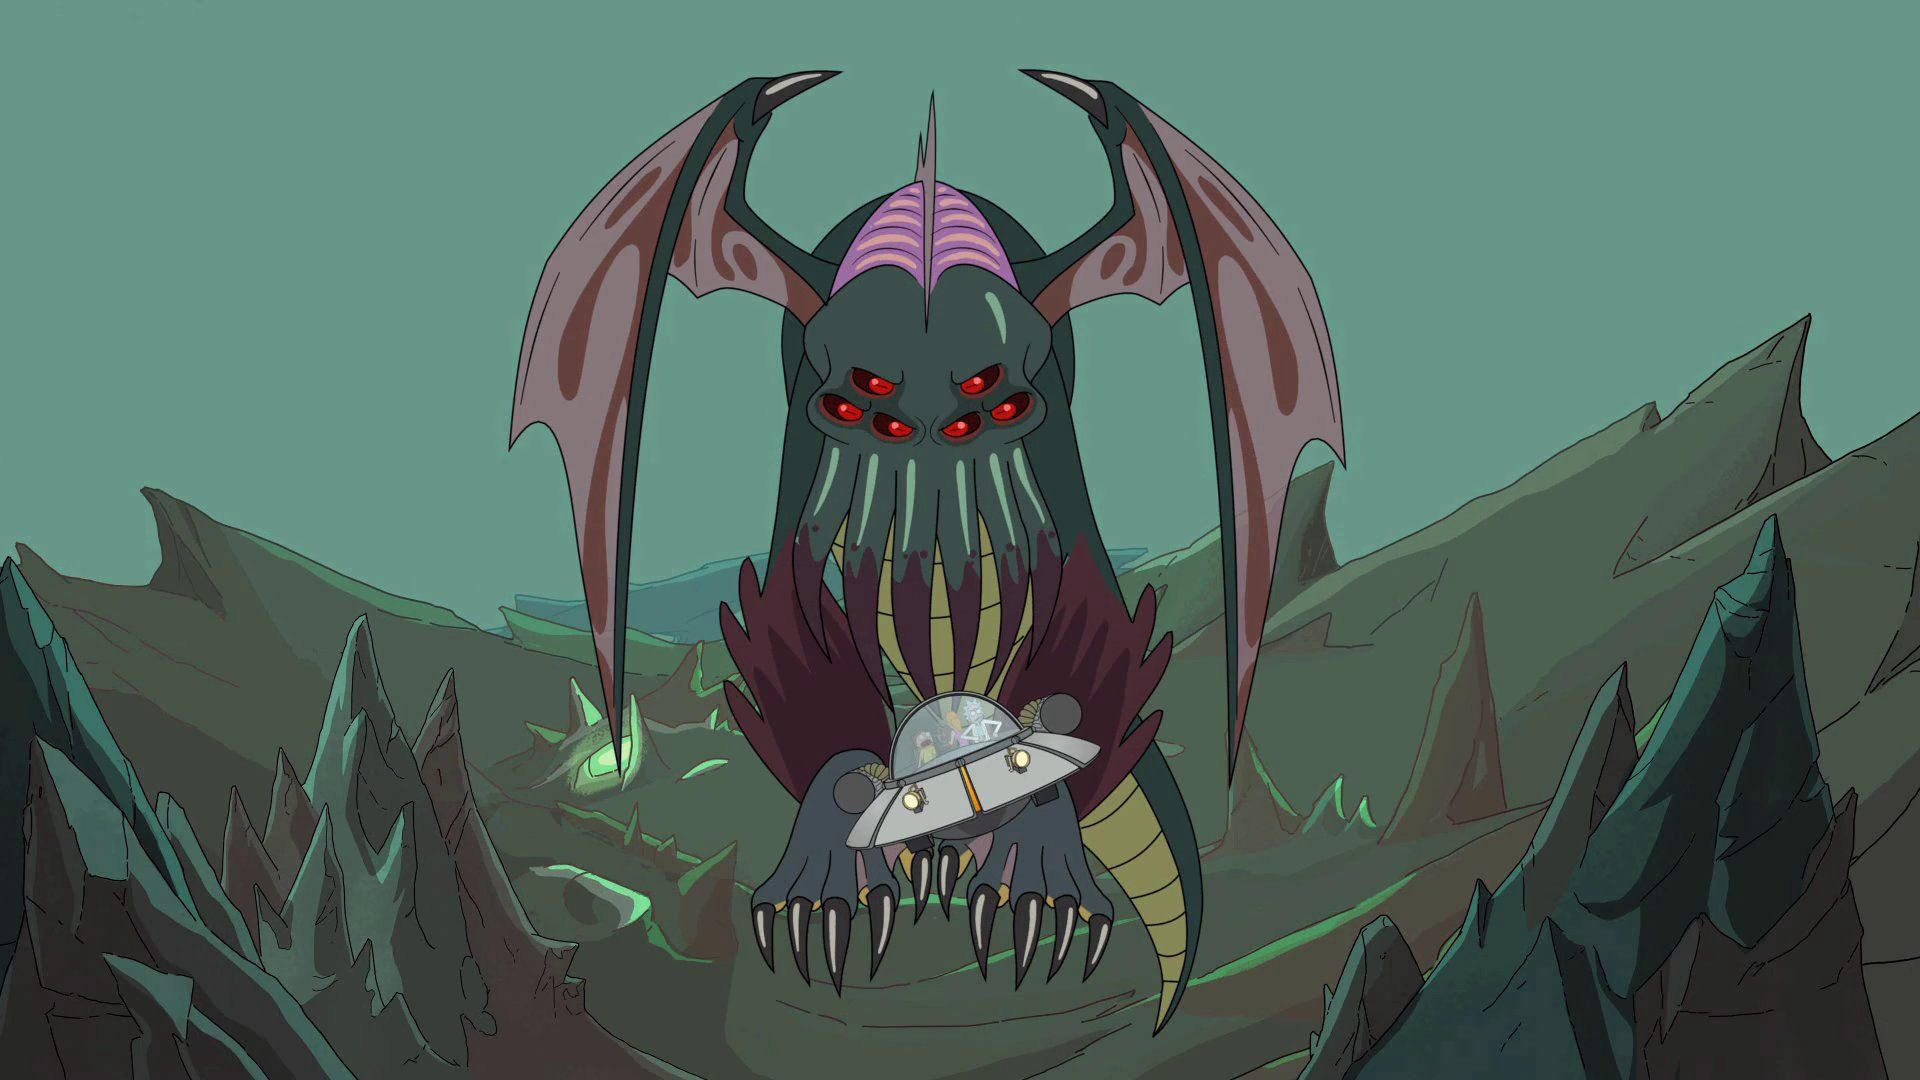
\includegraphics[scale=0.085]{kuvat/cthulhu parempi.jpg}
\pagebreak

\section{Rakkausseikkailu 2007}
\textit{Melodia: Veikkaan, että tiedät :D}

Maa kutsuu mä en vastaa.\\
Näen sinut ainoastaan.\\
Linnunradalla leimuaa,\\
kun tuhat aurinkoa loistaa.

Leijun halki avaruuden.\\
Löydän uuden ulottuvuuden.\\
Kaappaa mukaasi muukalainen,\\
ja vie mut tähtien taa.

Tämä on rakkausseukkailu 2007.\\
Olen odottanut pitkään,\\
ja toivon tämän kestävän.\\
Olen katsonut taivasta kohden,\\
ja toivonut enemmän.\\
Tää on seikkailuista valtavin.\\
mä syöksyn kanssasi halki galaksin.\\
Tämä on rakkausseukkailu 2007.

Taas lähtölaskenta alkaa.\\
En tottele painovoimaa.\\
Liekki syttyy raketti nousee,\\
taivasta tavoittamaan.

Leijun halki avaruuden.\\
Löydän uuden ulottuvuuden.\\
Kaappaa mukaasi muukalainen,\\
ja vie mut tähtien taa.

Tämä on rakkausseukkailu 2007.\\
Olen odottanut pitkään...

Olen odottanut pitkään...

Tämä on rakkausseukkailu 2007.

\columnbreak
\section{Kännimaa}

Kännimaahan lukkareilta moni tietä kysyy,\\
sinne saattaa löytää, vaikka pöydässänsä pysyy.\\
Katson snapsilasia ja ootan unohdusta,\\
sitsikansan teoissa on pala kadotusta.

Kännimaa on muutakin kuin pelkkää toiveunta.\\
Kännimaa on ihmismielen rauhan valtakunta.\\
Eikä sinne matka silloin kovin kauan kestä,\\
Kännimaa kun teekkarilta löytyy sydämestä!

Kännimaasta kuvitellaan paljon kaikenlaista,\\
kuinka miehet komistuu ja on niin satumaista.\\
Kun pöytäavec ongelmistaan koko illan jauhaa,\\
glögilasin pohjalta mä löydän mielenrauhaa!

Kännimaa on muutakin kuin alku sekä loppu.\\
Kännimaa on huoleton ja siellä ei oo hoppu.\\
Eikä meitä kukaan siellä ryyppäämästä estä,\\
kännimaa kun teekkareilta löytyy sydämestä!

\pagebreak

\section{Hauki ja muita ihmeitä}

Katonrajass’ kulkee hauki,\\
pahaa taitaa tarkoittaa!\\
:,: Kierrä pullon korkki auki,\\
ryyppy pedon karkoittaa. :,:

Pöydän alta ryömii lisko,\\
ilkein silmin tuijottaa.\\
:,: Ryyppy toinen naamaas kisko,\\
aistiharha lähdön saa. :,:

Vodka, vodka vill jag dricka,\\
jag vill äta kaviar.\\
:,: Jag vill älska russkij flicka,\\
jag vill spy i samovar! :,:

Koskenkorva vill jag dricka,\\
Jag vill gå på kräftkalas.\\
:,: Jag vill älska Suomi-neito,\\
jag vill spy i Aaltovas! :,:

\section{Huutolaatta}

Juon mä hiukan viinaa,\\
sitten oksennan, oksennan.\\
Vessaan ryömin,\\
sielläkin mä oksennan oksennan.\\
Huu-uutolaa-aatta,\\
huu-uutolaa-aatta.\\
Oksennan, oksennan.\\
Laatta se lennähtää.\\
Ei vittu kun iljettää.

Nyt tuntuu heikolta,\\
vatsassa kiertää taas.\\
Taidanpa piipahtaa,\\
mä nurkan takana.\\
Hetken jo helpottaa,\\
elämä voittaa taas.\\
Ei, olin väärässä!\\
Väistäkää, saatana!

Juon mä hiukan viinaa...
\columnbreak

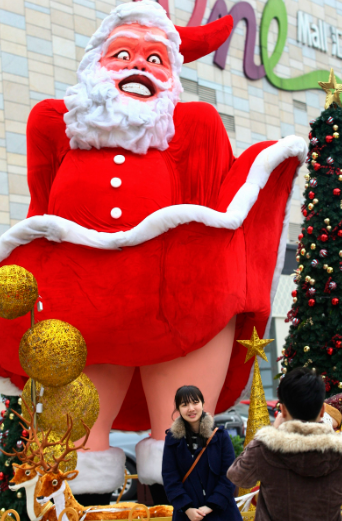
\includegraphics[scale=0.64]{kuvat/pukkijoulureisi.png}
\section{No onkos tullut joulu}
No onkos tullut kesä nyt talven keskelle?\\
:,: Ja laitetaankos pesä nyt pikkulinnuille? :,:

Jo kuusi kynttilöitä on käynyt kukkimaan.\\
:,: Pimeitä talven öitä nyt ehkä valaistaan. :,:

Ja vanhakin nyt nuortuu kuin lapsi leikkimään.\\
:,: Ja koukkuselkä suortuu, nyt kaikk' on mielissään. :,:

Lumi on jo peittänyt kukat laaksosessa,\\
järven Aalto jäätynyt talvipakkasessa.\\
Varpunen pienoinen, syönyt kesäeinehen,\\
järven Aalto jäätynyt talvipakkasessa.

:,: Joulu on nyt, joulu on nyt,\\
kattilat täynnä puuroo. :,:\\
:,: Nyt sitä saa, nyt sitä saa,\\
vatsansa täyteen puuroo. :,:
\vspace{0.5cm}

\input{laulut/jallutehdän-alla}

\hspace*{-4cm}
\includegraphics[scale=1.2]{kuvat/jallutahti.png}
\columnbreak
\section{Ken ompi phuksi}

;.: Who is a fuksi of Data Guild\\
stand up, stand up right now ;.:\\
Take you drink into your hand, then raise it up to your lips and\\
;.: Drink up, drink up, drink up, drink up,\\
drink your bottoms up ;.:

:,: Ken ompi fuksi PT:en\\
hän ylös nouskohon. :,:\\
Hän lasin käteen ottakoon\\
Sen huulillensa nostakoon.\\
:,: Juo pois, juo pois, juo pois, juo pois.\\
Juo herran tähden pois. :,:

:,: Ken ompi fuksi Inkubion\\
hän ylös nouskohon. :,:

:,: Ken ompi fuksi Athenen\\
hän ylös nouskohon. :,:

:,: Ken ompi fuksi AS:n\\
hän ylös nouskohon. :,:

:,: Ken ompi fuksi TiK:n\\
hän ylös nouskohon. :,:

:,: Ken ompi fuksi Prodekon\\
hän ylös nouskohon. :,:

:,: Ken ompi fuksi FK:n\\
hän ylös nouskohon. :,:

:,: Ken ompi fuksi SIK:n\\
hän ylös nouskohon. :,:

:,: Ken ompi fuksi KIK:n\\
hän ylös nouskohon. :,:

:,: Ken ompi fuksi IK:n\\
hän ylös nouskohon. :,:

:,: Ken ompi fuksi AK:n\\
hän ylös nouskohon. :,:

:,: Ken ompi fuksi MK:n\\
hän ylös nouskohon. :,:

:,: Ken ompi fuksi TF:n\\
hän ylös nouskohon. :,:

:,: Ken ompi FTMK 'nn\\
hän ylös nouskohon. :,:



\section{Paavi ja sulttaani}

On paavin elo ihanaa,\\
hän kaikki anerahat saa.\\
:,: On viini kallein juomansa\\
- Oi, jospa paavi oisin ma. :,:

Mutt' ei, ei koskaan maistaa saa,\\
hän nuoren naisen suudelmaa.\\
:,: Käy illoin yksin nukkumaan\\
- en paavi olla tahtoiskaan! :,:

Mutt' sulttaani hän hummailee\\
ja haaremissaan elelee.\\
:,: Keskellä naisten viehkeäin\\
- sulttaani oisin mielelläin. :,:

Mutt' ei, hän ompi polo mies\\
hänt' painaa Koraaninsa ies.\\
:,: Ei maista viinin tippaakaan\\
- en sulttaaniksi tahtoiskaan. :,:

En yksin olla tahtoisi\\
mä paavi enkä sulttaani.\\
:,: Mutt' vuoroin virkaan kumpaankin\\
mä mielelläni astuisin. :,:

Suo suukko mulle neitonen,\\
oon sulttaani mä hetkisen.\\
:,: Hei, veikot, maljat täyttäkää,\\
kun paaviks' muuttuu poika tää. :,:
\pagebreak
\end{flushleft}
\end{multicols}


\begin{center}
\pagebreak
\vspace*{1cm}

\pgfornament[scale=0.15]{80}
%viiva
\pgfornament[scale=0.25]{58}
%viiva
\pgfornament[scale=0.15]{80}

\vspace{1cm}
\section*{\hfill Ikuisen teekkarin laulu \hfill}

Talvi-iltain tummentuessa\\
Polin suojiin me saavumme taas.\\ 
:,: Meidät tekniikka jälkeen on jättänyt,\\
sen me tahdomme unhoittaa. :,:

Unelma vain on diplomityömme,\\
joka tenttimme vanhennut.\\
:,: Jo ruostunut harpikko käyttämätön,\\
tushi pulloihin jähmennyt. :,:

Aina teekkaripolvien uutten\\ 
ohi pöytämme käyvän nään\\
:,: Mutta meillä ei voimaa enää kylliksi\\
heidän joukkoonsa liittymään. :,:

Viini laseissa ilkkuen päilyy,\\
meitä kutsuen kuohuillaan. \\
:,: Pois murheemme tahdomme karkoittaa,\\
äly pois mitä maksoikaan! :,: 

Ja kun Integer vitae meille\\
kerran viimeisen lauletaan. \\
:,: Silloin ikuisen teekkarin haudalle\\ oluttynnöri nostetaan. :,: 
\vspace{1.3cm}

\pgfornament[scale=0.15]{80}
%viiva
\pgfornament[scale=0.25]{58}
%viiva
\pgfornament[scale=0.15]{80}
\newpage
\vspace*{2cm}

\hspace*{-2cm}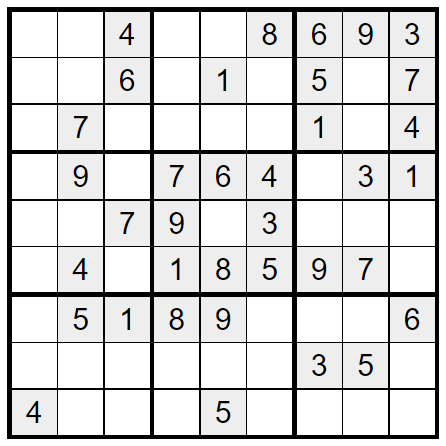
\includegraphics[scale=1.7]{kuvat/sudoku.png}
\\
\vspace{1cm}

\end{center}

\end{document}
